\documentclass[12pt,letterpaper,english]{article}
\usepackage[T1]{fontenc}
\usepackage[latin9]{inputenc}
\pagestyle{empty}
\usepackage{amsmath}
\usepackage{amssymb}
\usepackage{graphicx}
\usepackage{bm}
\usepackage{multicol}
\usepackage{enumitem}

\usepackage{hyperref}
\hypersetup{
    colorlinks=true,
    linkcolor=blue,
    filecolor=magenta,      
    urlcolor=cyan,
}

\newcommand{\norm}[1]{\lVert#1\rVert}

\makeatletter

\special{papersize=\the\paperwidth,\the\paperheight}



\textwidth6.5in\textheight9in\topmargin-.25in\oddsidemargin0in\evensidemargin0in\parskip5pt\parindent0pt


\usepackage{fancyhdr}
\pagestyle{fancy}
\lhead{Reconfigurable Mechanical Vibrations Laboratory Kit}
\rhead{}


\usepackage{lastpage}
 
 
\rfoot{Page \thepage \hspace{1pt} of \pageref{LastPage}}

%\rfoot{\small }
\lfoot{Mechanical Vibrations: Lab 1}

\cfoot{}




\usepackage{babel}


\makeatother

\usepackage{babel}
\begin{document}
\global\long\def\Re{{\rm {Re }}}
 \global\long\def\cL{{\cal L}}
 \global\long\def\sq{{\rm {sq}}}
 \global\long\def\bfx{{\bf x}}
 \global\long\def\bfi{{\bf i}}
 \global\long\def\bfj{{\bf j}}


\begin{center}
\textbf{\large Lab Assignment 1: 1DOF}
\par\end{center}{\large \par}

For this first lab assignment, you will investigate a forced 1 degree of freedom system. The system we will explore is a base excitation problem where a payload is forced by a spring attached to a vibrating base.  Part of the goal of this first assignment will be to help you get familiarized with the shaker setup, housing, and Matlab GUI that will be used for other labs in the future.  

\begin{center}
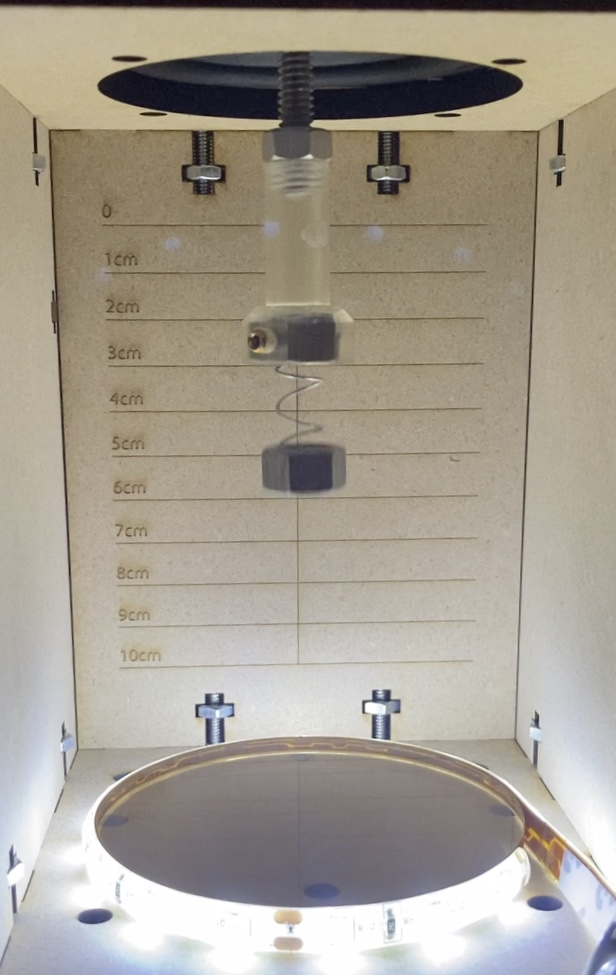
\includegraphics[width=2in]{lab1.jpg}
\end{center}

\begin{itemize}
\item In the Assembly Guide, first read through and complete the steps in sections A (Housing Assembly), B (Electronics Assembly), C (User Interface), D (Testing the System) to construct the shaker housing, assemble the simple electronic circuit for the shaker and learn to use the GUI.
\item Next read through subsections 1 and 1.1 under section E.  Subsection 1 is a general overview of how to use and assemble parts required for the first demo. Section 1.1 details the specific modifications to the general assembly that are needed for this week's demo. {\it Note that for this demonstration, we will not be using the linear shaft (as described in section E1).}
\end{itemize}

\begin{enumerate}
\item Take a picture of your completed setup.
\item We will first explore the effect of strobing.  For the best effect, the rest of the room should be reasonably dark. To do this, first attach only the nut to the spring (no magnets). Vibrate the speaker at 30Hz with a reasonable amplitude (ensuring that it's not bottoming out!). Then, activate the strobing option on the GUI. Initially, set the strobing frequency offset to 1Hz. Then, explore what happens as the strobing frequency offset is changed to larger or smaller values.  Describe and rationalize observations of the strobing effect you observe and the quantitative influence of the offset.
\item Based on the instructions in E1.1, we will explore the different regimes of forced vibration discussed in class. We will tune the mass of the payload by attaching one or two magnets to the nut. Predict the natural frequency of the three configurations (only nut, one magnet attached, two magnets attached). The spring constant is given by the manufacturer to be around 1050 N/m, while the mass of one nut is approximately 7 g. The mass of one magnet is around 12 g. 
\item We will first investigate the configuration where the nut and one magnet are attached to the end of the spring. Our goal is to use the help of strobing to sweep the frequency space and observe the effect of the driving frequency. For this, we recommend using an offset strobing frequency of 1 or 2 Hz. Start the sweep at around 10 Hz (the speaker is not designed to operate any lower). Then, increase the frequency in 5 Hz steps. As you are doing this, take note of the relative amplitude between the rigid mounting coupler and nut to get a sense of the magnification.  Also take note of the relative phase between the mounting coupler and nut. Continue the sweep in 5 Hz increments until you reach the predicted natural frequency.  You should see the largest amplification around this value since the system is only very weakly damped. Finally sweep beyond the natural frequency until you notice that the nut is almost stationary while the mounting coupler is still visibly vibrating.  Make a qualitative sketch/plot of the motion of the mass and mount as a function of time for three cases (clearly specifying the frequencies chosen): (1) Below the predicted natural frequency, (2) at the predicted natural frequency, and (3) above the natural frequency, again paying particular attention to the relative amplitude and phase of the driving and response.
\begin{itemize} 
\item {\small \underline{Tips:} During the sweep, you may notice that the nut has higher order resonant modes which causes the nut to vibrate side to side. If you encounter these modes, simply skip over that specific frequency (only vertical amplification constitutes the actual resonance we are looking for). 
\item As you sweep, be careful to tune the amplitude slowly so as to avoid the speaker bottoming out (this is when the threading piece glued to the speaker starts hitting the bottom of the speaker and can be easily identified from a clashing sound). As the frequency is increased, the max amplitude of the speaker decreases. Thus you will need to adjust the amplitude value on the GUI as frequency changes. 
\item If the lights start to dim during your sweep, simply reduce the amplitude of the shaker to 0 with the GUI, increase your computer's volume until the lights are at a suitable intensity, then slowly increase the shaker amplitude on the GUI again.
\item If you hear the speaker bottoming out, the fastest way to shutdown the system is to either mute your volume or immediately press the system off button on the GUI. }
\item {\small Ensure that the magnet is properly centered around the nut. This will help minimize any additional side to side vibrational modes. 
\item Be careful when handling the magnets so as to avoid them from snapping together quickly. The best way to remove them from one another once attached is to slide them apart tangentially as opposed to pulling them apart in the normal direction.  }

\end{itemize}



\item Repeat part (d) with no magnet, and finally with both magnets attached. 
\item Provide feedback or ideas (positive and/or areas for improvement) on the setup process and first 1DOF demonstration.  (Optionally) Please also share any other photos or videos you collect!
 
\end{enumerate}






\end{document}
